\documentclass
[
a4paper,                                                            % Papierformat
12pt,                                                                % Schriftgröße
oneside,                                                       % Zweiseitig
openright,                                                            % Neues Kapitel immer auf der rechten Seite
titlepage,                                                            % Titelseite
headinclude,                                                        % Seitengröße auch bei Kopfzeile
numbers=noenddot,                                                    % Bei Kapiteln keine abschließenden Punkte
listof=numbered,                                                    % Listingsverzeichnis
bibliography=totocnumbered,                                            % Literaturverzeichnis
]
{scrbook}                                                            % Dokumenttyp

\usepackage[bottom=1in,inner=1in,outer=20mm,top=20mm]{geometry}        % Ganze Seite verwenden

% Kopf und Fußzeile
\usepackage{emptypage}                                                % Leere Seiten ohne Kopf und Fußzeile
\usepackage[headsepline]{scrlayer-scrpage}                            % Kopf und Fußzeile
\pagestyle{scrheadings}                                                % Nummerierung in der Kopfzeile
\clearscrheadfoot                                                    % Kopf und Fußzeile löschen
\rehead{\headmark}                                                    % Kapitelname auf der geraden Seite innen
\ohead[\pagemark]{\pagemark}                                        % Seitennummerierung
\lohead{}                                                            % Name auf der ungeraden Seite innen
\renewcommand*{\chapterpagestyle}{scrheadings}                        % Kopf und Fußzeile auf Seiten mit Überschriften anders

% Dokumenteinstellungen und Paketimporte
\usepackage{lscape}
\usepackage[T1]{fontenc}                                            % Outputencoding
\usepackage{lmodern}
\usepackage[utf8]{inputenc}                                            % UTF8 + Sonderzeichen
\usepackage{newtxtext, newtxmath}                                    % Font Verbesserungen (z.B. µ direkt verwendbar)
\usepackage[ngerman]{babel}                                            % Deutsch
\usepackage{caption}                                                % Tabellen Listings und Figuren mit Beschriftung in Verzeichnissen
\usepackage[hyphens]{url}                                            % Zeilenumbruch bei URLs
\usepackage{graphicx}                                                % Bilder
\usepackage{float}                                                    % Plazierung von Floats (Bilder Tabellen)
\usepackage{wrapfig}                                                % Textumfluss von Bildern, die nicht die ganze Seite brauchen
\usepackage{setspace}                                                % Zeilenabstand
\usepackage{listings}                                                % Listings (=Code)	% Courier (listings)
\usepackage{times}                                                    % Schriftart Times Roman
\usepackage{courier}                                                % Schriftart Courier
\usepackage{array,multirow}                                            % Bessere Tabellenformatierung % Farben für Codehighlighting oder ähnliches
\usepackage{tabularx}                                                % Bessere Tabellen
\usepackage{appendix}                                                % Anhang Titelseite
\usepackage[printonlyused,withpage]{acronym}                        % Für die Verwendung von Akronymen + Verzeichnis - printonlyused: Abkürzung nur im Verzeichnis wenn auch benutzt; withpage: Seite der 1. Verwendung im Verzeichnis anzeigen
\usepackage[table,xcdraw]{xcolor}
\usepackage[normalem]{ulem}
\usepackage{tikz}
\usepackage{tikz-3dplot}
\useunder{\uline}{\ul}{}

\setlength{\parindent}{0em}                                            % Einrücken
\setcounter{tocdepth}{5}                                            % Tiefe der Überschriften
\setcounter{secnumdepth}{5}                                            % Nummerierungstiefe der Überschriften


\usepackage[bookmarks]{hyperref}                                    % Automatische Lesezeichen
\usepackage[figure]{hypcap}                                        % Bild referenzieren



\subject{\includegraphics[scale=0.7]{fig/logoMecha}}
\title{Diplomarbeit ReShuffled}

\subtitle{
HTBLA Kaindorf an der Sulm\\
Grazer Straße 202, A-8430 Kaindorf an der Sulm\\
Ausbildungsschwerpunkt Mechatronik}
\author{Vollmaier Alois \and Perl Nicolas \and Hörmann Stefan}
\date{Abgabedatum: 06.04.2020}
\publishers{
{Dr. Dipl-Ing. Gerhard Pretterhofer}\\ \vspace{0.2cm}
Dipl-Ing. Manfred Steiner}


\begin{document}
    \onehalfspace
    \maketitle
    \tableofcontents
    

\chapter{Einleitung}
\lohead{ReShuffled Projektplanung}

\section{Das Projektteam}
\label{sec:Einleitung}
\begin{figure}[H]
    \vspace{-30pt}
    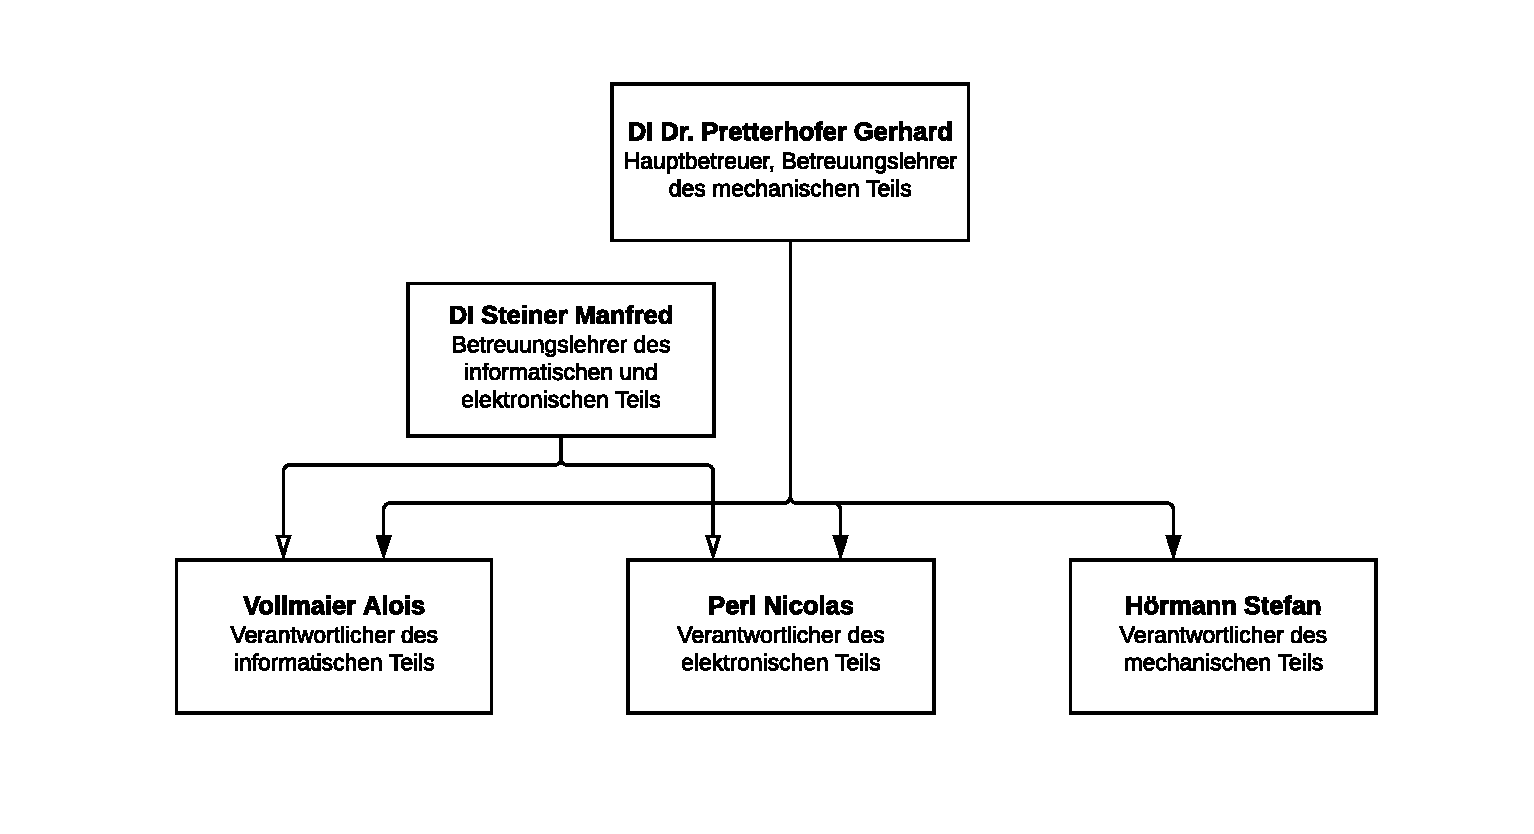
\includegraphics[width=0.80\textwidth]{fig/Hierachie_Reshuffled.pdf}
    \caption{Betreuerübersicht}
    \label{Bild über ganze Seitenbreite}
\end{figure}


\section{Konzept}
Wir setzten uns als Ziel eine Maschine zu entwickeln, welche das Mischen, sowie das Ausgeben von Spielkarten übernimmt.
Die Idee ist es, diese Verfahren möglichst platzsparend, zeiteffizient und detailliert durchdacht und optimiert zu realisieren.\\

\begin{wrapfigure}{r}{0.34\textwidth}
    \vspace{-40pt}
    \begin{center}
        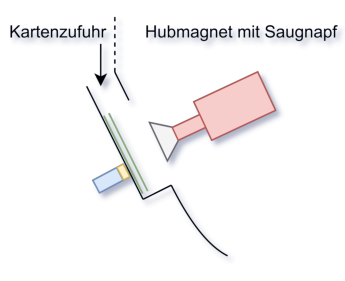
\includegraphics[width=0.35\textwidth]{fig/Reshuffled_Version_3_prinzip}
    \end{center}
    \caption{Kartenentnahme}
    \label{Kartenentnahme}
    \vspace{-15pt}
\end{wrapfigure}

Grundsätzlich basiert das Mischprinzip auf einer Art "Fächersystem".
Eingelegte Karten gelangen mithilfe eines ausgeklügelten Systems, welches aus einem Hubmagneten mit integriertem Saugnapf besteht, aus dem Einlegefach.
Erfolgt die Kartenentnahme, rutscht die Karte in ein zufälliges Fach des Lagerrads. Anschließend wird dieses Lagerrad in Drehbewegung versetzt um die gelagerten Karten auszugeben.

Der Benutzer steuert diese Maschiene auf einer GUI welche auf einem 7" LCD Display angezeigt wird. Systemintern steuert ein 8Bit Mikrocontroller der AVR-Familie den Ablauf.

%============================================
\chapter{Mechanik}
\lohead{Stefan Hörmann}
\label{sec:Mechanik}
\section{Beschreibung}

TODO


%============================================
\chapter{Elektronik}
\lohead{Nicolas Perl}
\label{sec:Elektronik}
\section{Beschreibung}

TODO



%============================================
\chapter{Informatik}
\lohead{Alois Vollmaier}
\label{sec:Informatik}
\section{Beschreibung}

Den Informatischen Teil der Arbeit kann man grundsätzlich in 2 Bereiche aufteilen. Einerseits soll eine einfache grafische Benutzeroberfläche gestaltet werden, auf welcher man den Mischvorgang steuern sowie grundlegende Einstellungen des Spieles vornehmen kann.
Aus programmtechnischen Gründen wird hierfür die Programmiersprache Java und das GUI-Toolkit Swing verwendet. \\
Die Hardwarekomponenten setzten sich aus einem Raspberry Pi 3B+ und einem 7" LCD Touchscreen der Firma Elecrow zusammen. \\

Andererseits besteht dieser Teilbereich der Arbeit auch aus der hardwarenahen Programmierung der Hauptplatine. Mithilfe der Programmiersprache C sollte der verbaute 8Bit Mikrocontroller der AVR-Familie namens ATmega 324P programmiert werden.
Dieser steuert den gesamten Ablauf der Maschiene. \\

Der Datenaustausch zwischen Hauptplatine und Raspberry PI erfolgt über die serielle Schnittstelle namens UART
{\itshape (Universal Asynchronous Receiver Transmitter)}
Hierfür wird die Open-Source-Bibliothek JSSC
{\itshape (Java Simple Serial Connector)}  verwendet.
%============================================
\chapter{Projektplanung}
\lohead{ReShuffled Projektplanung}
\label{sec:Projektplanung}
\section{Meilensteine}
\begin{table}[h!]
    \begin{tabular}{ll}
        \hline
        \rowcolor[HTML]{C0C0C0}
        \multicolumn{2}{c}{\cellcolor[HTML]{C0C0C0}\textbf{Meilensteine}}                      \\ \hline
        \rowcolor[HTML]{EFEFEF}
        \multicolumn{1}{l|}{\cellcolor[HTML]{EFEFEF}Datum} & Beschreibung                      \\ \hline
        \multicolumn{1}{l|}{15 Apr 2019}                   & Vollenden des Variantenvergleichs \\ \hline
        \multicolumn{1}{l|}{1 Jun 2019}                    & Fertigstellung der CAD Zeichnung  \\ \hline
        \multicolumn{1}{l|}{15 Sep 2019}                   & Fertigstellung der Hardware       \\ \hline
        \multicolumn{1}{l|}{31 Okt 2019}                   & Abschließen des Testaufbaus       \\ \hline
        \multicolumn{1}{l|}{1 Dez 2019}                    & Fertigstellung der Software       \\ \hline
    \end{tabular}
\end{table}

\section{Aufgabenplanung bis September}

Ziele des Herrn Hörmann:
\begin{itemize}
    \item Standartmäßig ist ein schwarzer Punkt davor.
    \item Die Länge ist nicht von Bedeutung, Zeilen werden automatisch umgebrochen.
\end{itemize}

\noindent\hrulefill

Ziele des Herrn Pearl:
\begin{itemize}
    \item Standartmäßig ist ein schwarzer Punkt davor.
    \item Die Länge ist nicht von Bedeutung, Zeilen werden automatisch umgebrochen.
\end{itemize}

\noindent\hrulefill

Ziele des Herrn Vollmaier:
\begin{itemize}
    \item Standartmäßig ist ein schwarzer Punkt davor.
    \item Die Länge ist nicht von Bedeutung, Zeilen werden automatisch umgebrochen.
\end{itemize}

%============================================
\chapter{Anhang}


\tikzset{isometricXYZ/.style={x={(-0.866cm,-0.5cm)}, y={(0.866cm,-0.5cm)}, z={(0cm,1cm)}}}
\tikzset{isometricZXY/.style={x={(0.866cm,-0.5cm)}, y={(0cm,1cm)}, z={(-0.866cm,-0.5cm)}}}
\tikzset{isometricYZX/.style={x={(0cm,1cm)}, y={(-0.866cm,-0.5cm)}, z={(0.866cm,-0.5cm)}}}
\begin{tikzpicture} [scale=4, isometricZXY, line join=round,
opacity=.75, text opacity=1.0,%
>=latex,
inner sep=0pt,%
outer sep=2pt,%
]

    \def\h{5}

    \newcommand{\quadrant}[2]{
    \foreach \t in {#1} \foreach \f in {175,165,...,5}
    \draw [fill=#2]
    ({sin(\f - \h)*cos(\t - \h)}, {sin(\f - \h)*sin(\t - \h)}, {cos(\f - \h)})
    -- ({sin(\f - \h)*cos(\t + \h)}, {sin(\f - \h)*sin(\t + \h)}, {cos(\f - \h)})
    -- ({sin(\f + \h)*cos(\t + \h)}, {sin(\f + \h)*sin(\t + \h)}, {cos(\f + \h)})
    -- ({sin(\f + \h)*cos(\t - \h)}, {sin(\f + \h)*sin(\t - \h)}, {cos(\f + \h)})
    -- cycle;
    }

    %Quadrants
    \quadrant{220,230,...,300}{black}
    \quadrant{-60,-50,...,20}{white}
    \quadrant{30,40,...,120}{black}
    \quadrant{130,140,...,210}{none}

    %Movement arrows
    \foreach \t in {225,235,...,295}
    \foreach \f in {50,40,...,0}
    \draw [red, opacity=1.0, ->, thick]
    ({sin(\f - \h)*cos(\t - \h)}, {sin(\f - \h)*sin(\t - \h)}, {cos(\f - \h)})
    -- ({(1 + 0.2*cos(90 - \f))*sin(\f - \h)*cos(\t - \h)},
    {(1 + 0.2*cos(90 - \f))*sin(\f - \h)*sin(\t - \h)},
    {(1 + 0.2*cos(90 - \f))*cos(\f - \h)});

    \foreach \t in {125,135,...,205}
    \foreach \f in {110,100,...,0}
    \draw [black, ->, thick]
    ({(1 + 0.2*cos(90 - \f))*sin(\f - \h)*cos(\t - \h)},
    {(1 + 0.2*cos(90 - \f))*sin(\f - \h)*sin(\t - \h)},
    {(1 + 0.2*cos(90 - \f))*cos(\f - \h)})
    -- ({sin(\f - \h)*cos(\t - \h)},{sin(\f - \h)*sin(\t - \h)},{cos(\f - \h)});
    \foreach \t in {35,45,...,115}
    \foreach \f in {130,120,...,0}
    \draw [red, opacity=1.0 ,->, thick]
    ({sin(\f - \h)*cos(\t - \h)}, {sin(\f - \h)*sin(\t - \h)}, {cos(\f - \h)})
    -- ({(1 + 0.2*cos(90 - \f))*sin(\f - \h)*cos(\t - \h)},
    {(1 + 0.2*cos(90 - \f))*sin(\f - \h)*sin(\t - \h)},
    {(1 + 0.2*cos(90 - \f))*cos(\f - \h)});

    \foreach \t in {-55,-45,...,25}
    \foreach \f in {130,120,...,0}
    \draw [black, ->, thick]
    ({(1 + 0.2*cos(90 - \f))*sin(\f - \h)*cos(\t - \h)},
    {(1 + 0.2*cos(90 - \f))*sin(\f - \h)*sin(\t - \h)},
    {(1 + 0.2*cos(90 - \f))*cos(\f - \h)})
    -- ({sin(\f - \h)*cos(\t - \h)},{sin(\f - \h)*sin(\t - \h)},{cos(\f - \h)});

    %Annotations
    \path ({1.5*sin(100)*cos(75)}, {1.5*sin(100)*sin(75)}, {1.5*cos(100)}) node [right] {Compression};
    \path ({1.5*sin(70)*cos(-15)}, {1.5*sin(70)*sin(-15)}, {1.5*cos(70)})  node [right] {Dilatation};
    \path ({1.25*sin(50)*cos(165)},{1.25*sin(50)*sin(165)},{1.25*cos(50)}) node [left]  {Dilatation};
    \path ({1.25*sin(30)*cos(255)},{1.25*sin(30)*sin(255)},{1.25*cos(30)}) node [left]  {Compression};

    %P and T axis
    \begin{scope}[ultra thick]
        \draw[->] ({1.75*sin(90)*cos(75)}, {1.75*sin(90)*sin(75)}, {1.75*cos(90)})
        -- ({2*sin(90)*cos(75)},{2*sin(90)*sin(75)},{2*cos(90)}) node [above] {T-axis};
        \draw[->] ({1.75*sin(90)*cos(255)},{1.75*sin(90)*sin(255)},{1.75*cos(90)})
        -- ({2*sin(90)*cos(255)},{2*sin(90)*sin(255)},{2*cos(90)}) node [below] {T-axis};
        \draw[<-] ({1.5*sin(90)*cos(-15)}, {1.5*sin(90)*sin(-15)}, {1.5*cos(90)})
        -- ({1.75*sin(90)*cos(-15)},{1.75*sin(90)*sin(-15)},{1.75*cos(90)}) node [right] {P-axis};
        \draw[<-] ({1.5*sin(90)*cos(165)}, {1.5*sin(90)*sin(165)}, {1.5*cos(90)})
        -- ({1.75*sin(90)*cos(165)},{1.75*sin(90)*sin(165)},{1.75*cos(90)}) node [left] {P-axis};
    \end{scope}

    % Label
    \node [anchor=north, yshift=-2mm] at (current bounding box.south)
    {Seismic focal mechanism and Pression-Tension axis.};
\end{tikzpicture}



\end{document}
